% ==============================================================================
%
%                             Mission
%
% ==============================================================================
\chapter{Mission} \label{chapt:mission}
The following sections will
first cover the starting point based on appendix \ref{app:aufgabenstellung} and the available resources (appendix \ref{app:technicial_requirements}). Different possible
solutions will be covered in \ref{chapt:solutions} before presenting the concept
in \ref{chapt:mission:concept}.
\\

In a world of self driving cars and virtual reality, having a digital copy of
the real world yields several benefits. Cars can be trained in a virtual city
to increase the performance of their algorithms and video games could get more
realistic if the player could walk through the streets of a major city. Gathering
this data is one problem and processing the images is another. Pictures have
to be converted, analyzed and processed. This requires a great deal of
computational power for a task that is repeated several times.

% ==============================================================================
%
%                             Starting Point
%
% ==============================================================================
\section{Starting Point}
To accelerate intense image processing a dedicated hardware approach is
investigated. To do so, a basic image processing algorithm such as edge
detection is implemented in an FPGA that communicates over a network with a host
computer. The image processing task should later be distributed onto multiple
FPGAs to accelerate the processing even more \cite{nomokoReqs}. Before listing possible solutions the available resources need to
be dissected.

\subsection{FPGA Board} \label{chapt:fpgaboard}
\begin{figure}[tb!]
    \centering
    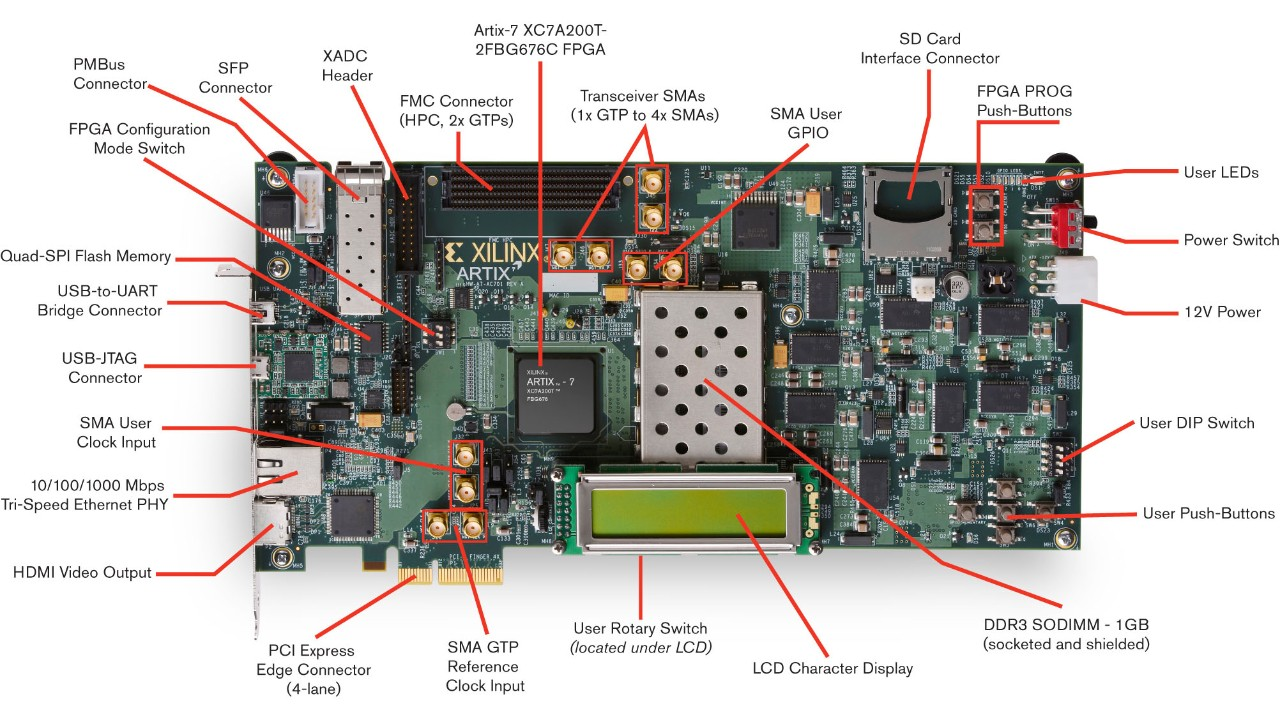
\includegraphics[width=\textwidth]{images/mission/ac701.png}
    \caption{Xilinx AC701 Evaluation Kit \cite{image_ac701}}
    \label{fig:ac701}
\end{figure}

The Xilinx AC701 Evaluation Kit is used as development platform. It features an
Artix-7 FPGA and several useful on-board peripherals. The JTAG interface is used
for configuration and debugging of the FPGA. To connect the platform to the
network, a Gigabit Ethernet PHY handles the first layer of the OSI model in
hardware (see chapter \ref{chapt:physical}). Storing data is possible in the DDR3 memory
module. Table \ref{tab:ac701} shows a summary of the important peripherals on
the AC701 board.
\\
\begin{table}[b!]
    \centering
    \begin{tabular}{l l}
        \toprule
        Part & Description \\
        \midrule
        FPGA & XC7A200T-2FBG676C \\
        JTAG & Onboard JTAG configuration circuitry to enable configuration over USB \\
        Memory & DDR3 SODIMM 1GB up to 533MHz / 1066Mbps \\
        Ethernet & 10/100/1000 Mbps Ethernet (RGMII) \\
        \bottomrule
    \end{tabular}
    \caption{Xilinx AC701 key board features \cite{xilinx_ac701}}
    \label{tab:ac701}
\end{table}

The XC7A200T FPGA is part of the Artix-7 family. It is optimized for high logic
throughput at low costs. Important for this project is the number of logic cells
and the amount of on-chip memory. With more logic cells available, data can be
processed parallel and the throughput increases. Processing more data at the
same time also requires the data to be stored. Therefore on-chip memory, also
called block memory, is used to have fast access to the data. Table 
\ref{tab:XC7A200T} lists the relevant numbers of resources.

\begin{table}[tb!]
    \centering
    \begin{tabular}{l l}
        \toprule
         & XC7A200T \\
        \midrule
        Logic Cells & 215k \\
        DSP Slices & 740 \\
        Block Memory & 1642 KB \\
        \bottomrule
    \end{tabular}
    \caption{XC7A200T key features \cite{xilinx_ac701}}
    \label{tab:XC7A200T}
\end{table}

\subsection{Communication} \label{chapt:mission:communication}
The communication between host computer and FPGA is built up over Ethernet.
This way, the system can be expanded quickly and it requires little effort to
implement the communication on the computer.

Connecting multiple boards and a host computer on a network requires a network
switch. A switch analyzes the information stored in the Ethernet header (sender
and receiver MAC address) and forwards the package to the proper port. For this
system to work, the Ethernet protocol has to be implemented in the FPGA.

\begin{figure}[h]
    \centering
    % \tikzsetnextfilename{system-overview}
\begin{tikzpicture}[
    rounded corners=0mm,
]
    %coordinates
    
    %nodes

    \begin{pgfonlayer}{main}
        % PC
        \node[draw, fill=white, minimum width=3cm, minimum height=1cm, anchor=west, align=center] 
            (pc) at (0,0) {PC/server};
        % Switch
        \node[draw, fill=white, minimum width=3cm, minimum height=1cm, anchor=west, align=center, right=3cm of pc] 
            (switch) {10G switch};

        % FPGA1
        \node[draw, fill=white, minimum width=3cm, minimum height=1cm, anchor=west, align=center, below=1cm of switch, xshift=-5.5cm] 
            (f1) {FPGA};
        % FPGA2
        \node[draw, fill=white, minimum width=3cm, minimum height=1cm, anchor=west, align=center, right=0.5cm of f1] 
            (f2) {FPGA};
        % Dot
        \node[circle,fill=black,minimum size=0.2cm,inner sep=0pt, right = 0.5cm of f2] (dt1)  {};
        \node[circle,fill=black,minimum size=0.2cm,inner sep=0pt, right = 0.2cm of dt1] (dt2)  {};
        % FPGA3
        \node[draw, fill=white, minimum width=3cm, minimum height=1cm, anchor=west, align=center, right=0.5cm of dt2] 
            (f3) {FPGA};

        % PC to switch
        \path[draw,{Latex[length=2.5mm]}-{Latex[length=2.5mm]}] ($(pc.0) + (0,0)$) -- ($(switch.180) + (0,0)$)
            node[midway, above] () {10Gb/s} ;

        % Switch to f1
        \path[draw,-] 
            ($(switch.270) + (-1,0)$) |- ($(f1.90) + (0,0.6)$) -- ($(f1.90) + (0,0)$)
            node[midway, above] () {} ;
        % Switch to f2
        \path[draw,-] 
            ($(switch.270) + (-0.7,0)$) |- ($(f2.90) + (0,0.4)$) -- ($(f2.90) + (0,0)$)
            node[midway, above] () {} ;
        % Switch to f3
        \path[draw,-] 
            ($(switch.270) + (1,0)$) |- ($(f3.90) + (0,0.6)$) -- ($(f3.90) + (0,0)$)
            node[midway, above] () {} ;

        % 10G ellipse
        \draw[line width = 0.5mm] ($(switch.180) + (0,0)$) ellipse (0.2cm and 0.4cm);
        % 1G ellipse
        \draw[line width = 0.5mm] ($(switch.270) + (0,0)$) ellipse (1.2cm and 0.2cm);
        
        % 10G desc arrow
        \path[draw,-] 
            ($(switch.180) + (-0.1,0.3) + (-1,0.8)$) -- 
            ($(switch.180) + (-0.1,0.3)$)
            node[near start, above, anchor=south east,xshift=-0.3cm] () {10Gb/s uplink} ;
        % 1G desc arrow
        \path[draw,-] 
            ($(switch.270) + (1.0,0.1) + (1,0.8)$) -- 
            ($(switch.270) + (1.0,0.1)$)
            node[near start, above, anchor=south west,xshift=0.3cm] () {1Gb/s downlink} ;
        % Braces
            \draw [line width=0.5mm,decorate,decoration={brace,amplitude=10pt},xshift=-0pt,yshift=0pt] 
            ($(f3.0) + (0.5,-0.8)$) -- ($(f1.180) + (-0.5,-0.8)$)
            node [black,midway,yshift=-0.5cm,anchor=north] {$N_F=10$};
    \end{pgfonlayer}

    % FPGA box
    \begin{pgfonlayer}{main}
        % \node[above = 0.2cm of com, xshift=-1.5cm] (fpga) { FPGA };
    \end{pgfonlayer}
    \begin{pgfonlayer}{foreground}
        % \node (f_fpga) [draw=black, fill=gray!20, inner sep=20, fit={(com) (ip) }] {};
    \end{pgfonlayer} 

    
    

\end{tikzpicture}
    \caption{FPGA Network}
    \label{fig:fpganetwork}
\end{figure}
% To send and receive packets from and to a computer, it is preferable to use the
% internet protocol (IP). Sending data over UDP or TCP requires only a few lines
% of code. 
% kommunikation von PC auf den FPGA und zurück ist über ethernet zu realisieren 

\subsection{Image} \label{chapt:image}
Section \ref{chapt:fpgaboard} shows that the FPGA only has 1642 KB block memory. Therefore, it is important to know how large the image is. The file size of a 1500MPixel image with 24bit RGB values is calculated in the following equation:

\begin{equation}
	File Size = Pixel_{tot} * Pixel_{size} = 1500MPixel * 24bit = 36Gbit \cong 4.4GByte
    \label{eq:filesize}
\end{equation}

As shown in equation \ref{eq:filesize} a picture does not have space on the FPGA. The image must therefore be processed piecewise in the FPGA. 
The images to be processed have the format TIFF or DNG. 
\\

\textbf{TIFF (Tagged Image File Format):}
TIFF files can be divided into three sections, the Image File Header (IFH), the Image File Directory (IFD) and the bitmap data. The IFH and  IFD are mandatory in every TIFF file. The bitmap data is not essential. 
The IFH is constant in each TIFF file and consists of eight bytes. It is composed of the byte order, the special number 42 and an offset to the first IFD.
Visible in figure \ref{fig:tiff_format}, several images can be stored in a TIFF file and thus consist of several IFDs. The IFD contains information about an image. This information consists of tags that describe, for example, the width or the color system of the image. At the end of the IFD is the offset to the next IFD \cite{tiff_format}.
\\

\begin{figure}[tb!]
    \centering
    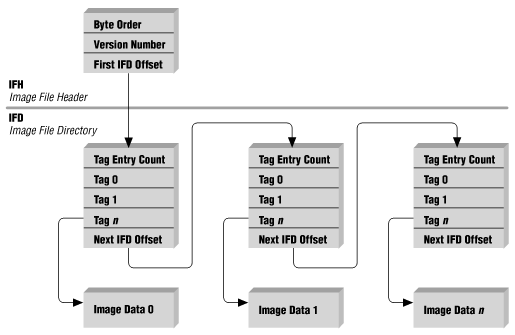
\includegraphics[width=0.9\textwidth]{images/mission/tiff_format.png}
    \caption{TIFF file format \cite{tiff_format}}
    \label{fig:tiff_format}
\end{figure}

\textbf{DNG (Digital Negative):}
DNG is a lossless raw data format by Adobe. It is compatible with the format and the standard of TIFF 6.0. It can also be saved with the file extension *. tif \cite{dng_format}. 
The TIFF 6.0 format differs from the previous formats mainly in the tags \cite{tiff_format}.

\subsection{Development Environment}
The image processing algorithm is written in Vivado HLS. With Vivado HLS, an IP core for the Vivado HLx can be generated from a C/C++ code. Vivado HLS is useful when programming algorithms and afterwards translating them into hardware description language. 
\clearpage
% ==============================================================================
%
%                             Possible Solutions
%
% ==============================================================================
\section{Possible Solutions} \label{chapt:solutions}
\subsection{Image Processing} \label{chapt:mission_imageprocessing}
There are many different image processing algorithms. However, it is important to filter the different algorithms and decide which one is meaningful and has a big advantage. The chapter \ref{chapt:theroy_imageprocessing} lists the three image processing operations and how many pixels of an image are required for processing. It's a good start to narrow down the algorithms.
\\

\textbf{Global Operations:} This requires the entire image. Chapter \ref{chapt:image} shows that there is not enough memory on the FPGA for the whole image. This operation is not suitable in this case.
\\

\textbf{Point Operations:} This operation is conceivable. However, it is quite undemanding and poorly shows which advantages a distributed FPGA system has. 
\\

\textbf{Neighborhood Operations:} In image analysis, it is helpful if edges, corners or objects can be detected. With these keywords you will find Feature Detection. Feature detection is a collection of algorithms which contain edges, corners, regions of interest, points or ridges. From all these different types, edge detection is most useful for image analysis. Edge detection can be used to detect objects (houses, windows, etc.).
With edge detection, the Sobel filter is a simple algorithm which is used frequently. The Sobel filter is also a basic building component for very good edge detection, such as canny edge detection \cite{canny_edge}. Altough it is not the best edge detector, it is very promising for setting up and testing the entire system.

\subsection{Communication} \label{chapt:mission:possible:communication}
% Die Vor- und Nachteile folgender Punkte werden aufgezeigt:
% UDP, TCP, fertige IPs, bestehende Protokolle
As mentioned in chapter \ref{chapt:mission:communication} a part of the OSI
model must be managed by the FPGA. The first layer is handled by the
on-board PHY chip but the data link, network, transport and session layers have
to be operated by the FPGA. Per layer the following options may be considered:
\\

\textbf{Own Implementation:}
The functionality is developed from scratch in hardware description language.
This method requires the most time of the three options. But in advance, the
functionality can be implemented exactly to the needs.
\\

\textbf{Opencore:} \url{https://opencores.org/} is a community for the
development of IP (Intellectual Properties) Cores. An IP Core is a piece of code
that can be used in an FPGA design. It advertises specific functionality and is
tested to certain specifications. The code is open source licensed and free to
use. Disadvantages are the uncertainty about the proper operation and the
portability to a specific FPGA.
\\

\textbf{Xilinx IP Core:} The FPGA manufacturer offers ready to use IP Cores.
They can be quickly added to the design because they are part of the development
environment. These cores are tested by the manufacturer and often come with an
example design for the evaluation kit. In disadvantage these cores often come at
a price and require a license.
\\

Table \ref{tab:commsol} lists the layers to be implemented and the possible
solutions that may be considered. The underlaying layer of the Data Link layer
does not feature any data buffering. Therefore the implementation of the Data
Link layer is time-critical. Xilinx offers the Tri-Mode Ethernet Media Access
Controller (TEMAC) \cite{temac}. It is suited for Gigabit Ethernet communication
and offers an example design for the AC701 evaluation kit. This solution is
chosen to omit the critical timing requirements and because it works out of the
box. 
To manage the tasks of the Network and Transport layers the 1G eth UDP / IP Stack
from \url{https://opencores.org/} is picked \cite{udpipstack}. It implements the
UDP and IPv4 protocols and couples directly to the TEMAC. UDP was chosen for
transport protocol because it does not require a handshake to establish a
connection which means less implementation effort. 

Finally, the Session layer is custom implemented. A lightweight file transfer
protocol on top of UDP that is suitable for efficient implementation
on FPGA is required. This is very application specific and therefore no suitable IP Cores
exist.

\begin{table}[h!]
    \centering
    \begin{tabular}{l l l l l}
        \toprule
        Layer & Protocol & Possible Solutions & & \\
        \midrule
        Data Link & Ethernet & 
        Own implementation & Opencore & Xilinx Core
        \\
        Network & IPv4 &
        Own implementation & Opencore & 
        \\
        Transport & TCP or UDP &
        Own implementation & Opencore & 
        \\
        Session & {} &
        Own implementation & &
        \\
        \bottomrule
    \end{tabular}
    \caption{Communication layer possible solutions}
    \label{tab:commsol}
\end{table}

% ==============================================================================
%
%                             Concept
%
% ==============================================================================
\clearpage
\section{Concept} \label{chapt:mission:concept}
Having compared the possible solutions for both the image processing and
communication part, the way of proceeding can be concluded.
\\

\textbf{Image Processing}
    \begin{itemize}
        \item Use high level synthesis
        \item Describe the processing task in C/C++
        \item Implement a Sobel filter
        \item Read and write data from FPGA block memory
    \end{itemize}

\textbf{Communication} 
    \begin{itemize}
        \item Use the Xilinx Tri-Mode Ethernet MAC for layer 2
        \item Use the 1G eth UDP / IP Stack from 
        \url{https://opencores.org/} for layer 3 and 4
        \item Define a custom layer 5 protocol and implement it accordingly
        \item Read and write data from FPGA block memory
    \end{itemize}

Figure \ref{fig:blockdiagram} shows the top level block diagram. The image data
is sent over Ethernet to the AC701 evaluation board. The on board PHY handles
layer 1 of the OSI model before passing the data to the FPGA. The communication
stack handles the file transfer and stores the data in FPGA block memory. The
image processing block then runs its task and the communication block sends the
data back to the computer.

\begin{figure}[h!]
    \centering
    % \tikzsetnextfilename{system-overview}
\begin{tikzpicture}[
    rounded corners=0mm,
]
    %coordinates
    \coordinate (corig)      at (0,0);
    \coordinate (cmonitor)   at (0,0);
    \coordinate (ccom)       at (5,0);
    \coordinate (cip)        at (10,0);


    %nodes

    \begin{pgfonlayer}{main}
        \node[draw, fill=white, minimum width=3.2cm, minimum height=1.8cm, anchor=west, align=center, rounded corners=1mm] (mon) at (cmonitor) {};

        \node[draw, fill=white, minimum width=2.1cm, minimum height=0.4cm, anchor=west, align=center, rounded corners=2mm, below=0.2cm of mon] (stand) {};
        \node[draw, fill=white, minimum width=0.2cm, minimum height=0.1cm, anchor=south, align=center] (stange) at ($(stand.90) + (0,-0.04)$) {};



        \node[draw, fill=white, minimum width=3cm, minimum height=1cm, anchor=west, text width=2.8cm, align=center, right = 2cm of mon] (com) at (ccom) {Communication};
        \node[draw, fill=white, minimum width=3cm, minimum height=1cm, anchor=west, text width=2.8cm, align=center, right = 1cm of com] (mem)  {Memory};
        \node[draw, fill=white, minimum width=3cm, minimum height=1cm, anchor=west, text width=2.8cm, align=center, below = 1cm of mem] (control)  {Controller};

        \node[draw, fill=white, minimum width=3cm, minimum height=1cm, anchor=west, text width=2.8cm, align=center, left = 1cm of control] (ip) {Image\\Processing};
        

        \node[inner sep=0pt, anchor=west] (whitehead) at ($(cmonitor) + (0.1,0)$)
            {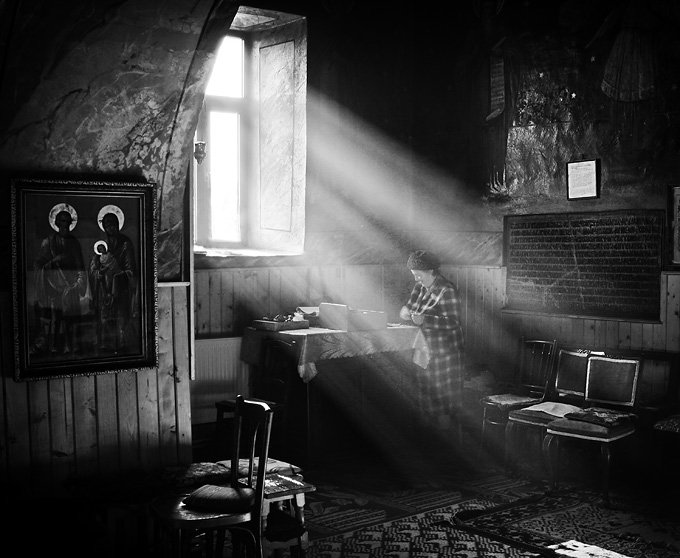
\includegraphics[width=1.4cm]{images/mission/room.png}};
        \node[inner sep=0pt, anchor=west] (whitehead) at ($(cmonitor) + (1.7,0)$)
            {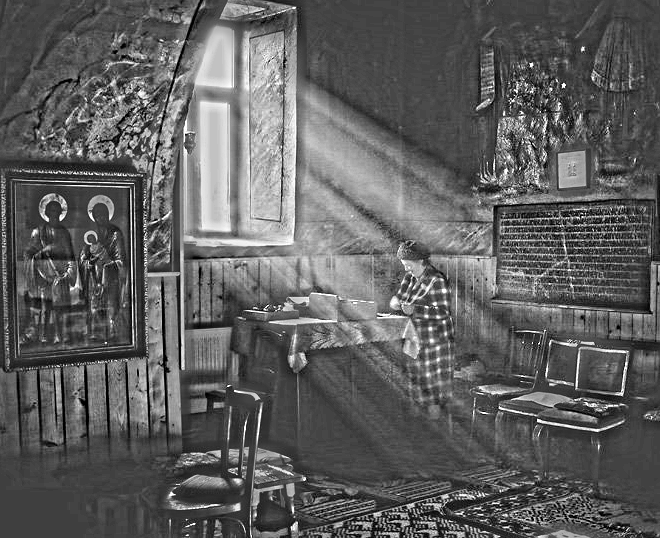
\includegraphics[width=1.4cm]{images/mission/room_fpga_vhdl_v20.png}};

        \node[] (eth) at ($(cmonitor) + (4.5, 1.0)$) {LAN};
        
        \draw[line width = 0.5mm] ($(eth) + (0,-1.0)$) ellipse (0.2cm and 0.5cm);
    \end{pgfonlayer}

    % FPGA box
    \begin{pgfonlayer}{main}
        \node[above = 0.2cm of com, xshift=-1.5cm] (fpga) { FPGA };
    \end{pgfonlayer}
    \begin{pgfonlayer}{foreground}
        \node (f_fpga) [draw=black, fill=gray!20, inner sep=20, fit={(com) (ip) (mem) (control) }] {};
    \end{pgfonlayer} 

    
    \path[draw,-{Latex[length=2.5mm]}] ($(mon.0) + (0,0.2)$) -- ($(com.180) + (0,0.2)$) node[near end, above] () {1.} ;
    \path[draw,{Latex[length=2.5mm]}-] ($(mon.0) + (0,-0.2)$) -- ($(com.180) + (0,-0.2)$) node[near end, below] () {8.} ;

    \path[draw,-{Latex[length=2.5mm]}] ($(control.180) + (0,0.2)$) -- ($(ip.0) + (0,0.2)$) node[midway, above] () {4.} ;
    \path[draw,{Latex[length=2.5mm]}-] ($(control.180) + (0,-0.2)$) -- ($(ip.0) + (0,-0.2)$) node[midway, below] () {5.} ;

    \path[draw,-{Latex[length=2.5mm]}] ($(control.90) + (-0.2,0)$) -- ($(mem.270) + (-0.2,0)$) node[midway, left] () {6.} ;
    \path[draw,{Latex[length=2.5mm]}-] ($(control.90) + (0.2,0)$) -- ($(mem.270) + (0.2,0)$) node[midway, right] () {3.} ;

    \path[draw,-{Latex[length=2.5mm]}] ($(com.0) + (0,0.2)$) -- ($(mem.180) + (0,0.2)$) node[midway, above] () {2.} ;
    \path[draw,{Latex[length=2.5mm]}-] ($(com.0) + (0,-0.2)$) -- ($(mem.180) + (0,-0.2)$) node[midway, below] () {7.} ;

\end{tikzpicture}
    \caption{Block diagram}
    \label{fig:blockdiagram}
\end{figure}


